\documentclass[a0,draft,portrait]{a0poster}
\usepackage{graphicx,color}
\pagestyle{empty}
\setcounter{secnumdepth}{0}
\usepackage[absolute]{textpos}
\usepackage{wrapfig,times}
\definecolor{DarkBlue}{rgb}{0.1,0.1,0.5}
\definecolor{Red}{rgb}{0.9,0.0,0.1}

% see documentation for a0poster class for the size options here
\let\Textsize\normalsize
\def\Head#1{\noindent\hbox to \hsize{\hfil{\LARGE\color{DarkBlue} #1}}\bigskip}
\def\LHead#1{\noindent{\LARGE\color{DarkBlue} #1}\smallskip}
\def\Subhead#1{\noindent{\large\color{DarkBlue} #1}}
\def\Title#1{\noindent{\VeryHuge\color{Red} #1}}

% Set up the grid
\TPGrid[40mm,40mm]{17}{25} % 5 - 1 - 5 - 1 - 5 Columns 

% Mess with these as you like
\parindent=0pt
%\parindent=1cm
\parskip=0.5\baselineskip

% The background
\usepackage{eso-pic}
%-----------------------------
\makeatletter
\newcommand\BackgroundPicture[2]{%
  \setlength{\unitlength}{1pt}%
  \put(0,\strip@pt\paperheight){%
  \parbox[t][\paperheight]{\paperwidth}{%
    \vfill
    \centering\includegraphics[angle=#2, width = 1.05\textwidth]{#1}
    \vfill
}}} %
\makeatother
\AddToShipoutPicture{\BackgroundPicture{figures/background_blank.pdf}{0}}  

\begin{document}
%HEADING:
\begin{textblock}{15}(0,0)
\begin{center}
\baselineskip=3\baselineskip \Title{Title}
\\
\vspace{1cm}
\LHead{\underline{Stig R. Jensen}$^{^1}$}\\
$^1$ Centre for Theoretical and Computational Chemistry, 
UiT - The Arctic University of Norway, NO-9037 Troms{\o}, Norway \\
\vspace{1cm}
\end{center}
\end{textblock} 

%Horizontal line:
\begin{textblock}{17}(0,3.5)
\begin{center}
 \hrule
\end{center}
\end{textblock}

%Logo 1:
\begin{textblock}{2.5}(14.5,0)

\includegraphics[width = \textwidth]{figures/uit.pdf} % or uio.pdf
\end{textblock} 

%Logo 2:
\begin{textblock}{2.5}(0,23.3)

\includegraphics[width = \textwidth]{figures/sff.pdf}
\end{textblock}

%Logo 3
\begin{textblock}{12}(5.3,23.4)

\includegraphics[width = \textwidth]{figures/ctcc.pdf}
\end{textblock}

% First column

\begin{textblock}{5}(0,4)
\LHead{Introduction}
\end{textblock}


\begin{textblock}{5}(0,7.8)
\LHead{The multiwavelet basis}

The multiwavelet basis consists of two types of polynomial bases
\end{textblock}

\begin{textblock}{5}(0.3,8.4)
\begin{itemize}
	\item Scaling functions
\end{itemize}
\end{textblock}

\begin{textblock}{5}(3,8.4)
\begin{itemize}
	\item Wavelet functions
\end{itemize}
\end{textblock}

\begin{textblock}{5}(0,9.0)
A projection onto the scaling basis at scale $N$ gives an approximation 
with polynomial grid cells of resolution $2^{-N}$.
\begin{equation}
	f(x) \approx f^N(x) 
\end{equation}
The wavelet projections $df^n$ are defined as the \emph{difference} between
two consecutive scaling projections.
\begin{equation}
	\label{eq:wavelet}
	df^n(x) = f^{n+1}(x) - f^n(x)
\end{equation}
By recursive application of eq. (\ref{eq:wavelet}) we have an alternative
\emph{multiresolution} representation of the approximation $f^N$.
\begin{equation}
	\label{eq:multires}
	f(x) \approx f^N(x) = f^{0}(x) + \sum_{n=0}^{N-1} df^n(x)
\end{equation}
\end{textblock}

% Second column

\begin{textblock}{5}(6,4.0)
\LHead{Section}

\end{textblock}

\begin{textblock}{5}(6,9.1)
\LHead{Section}

\Subhead{Subsection}
\end{textblock}

\begin{textblock}{5}(6,18.4)
\LHead{Section}

\end{textblock}


% Third column

\begin{textblock}{5}(12,4)
\LHead{Results}

\end{textblock}


\begin{textblock}{5}(12,15.0)
\LHead{Conclusions}

\end{textblock}


\begin{textblock}{5}(12,18.5)
% Change the reference heading style:
\renewcommand\refname{\textnormal{\LHead{References}}}

\bibliography{poster}
%\bibliographystyle{abbrv}
\bibliographystyle{plain}
\end{textblock}

%Figures

\begin{textblock}{5}(0,19.6)
  \begin{center}
    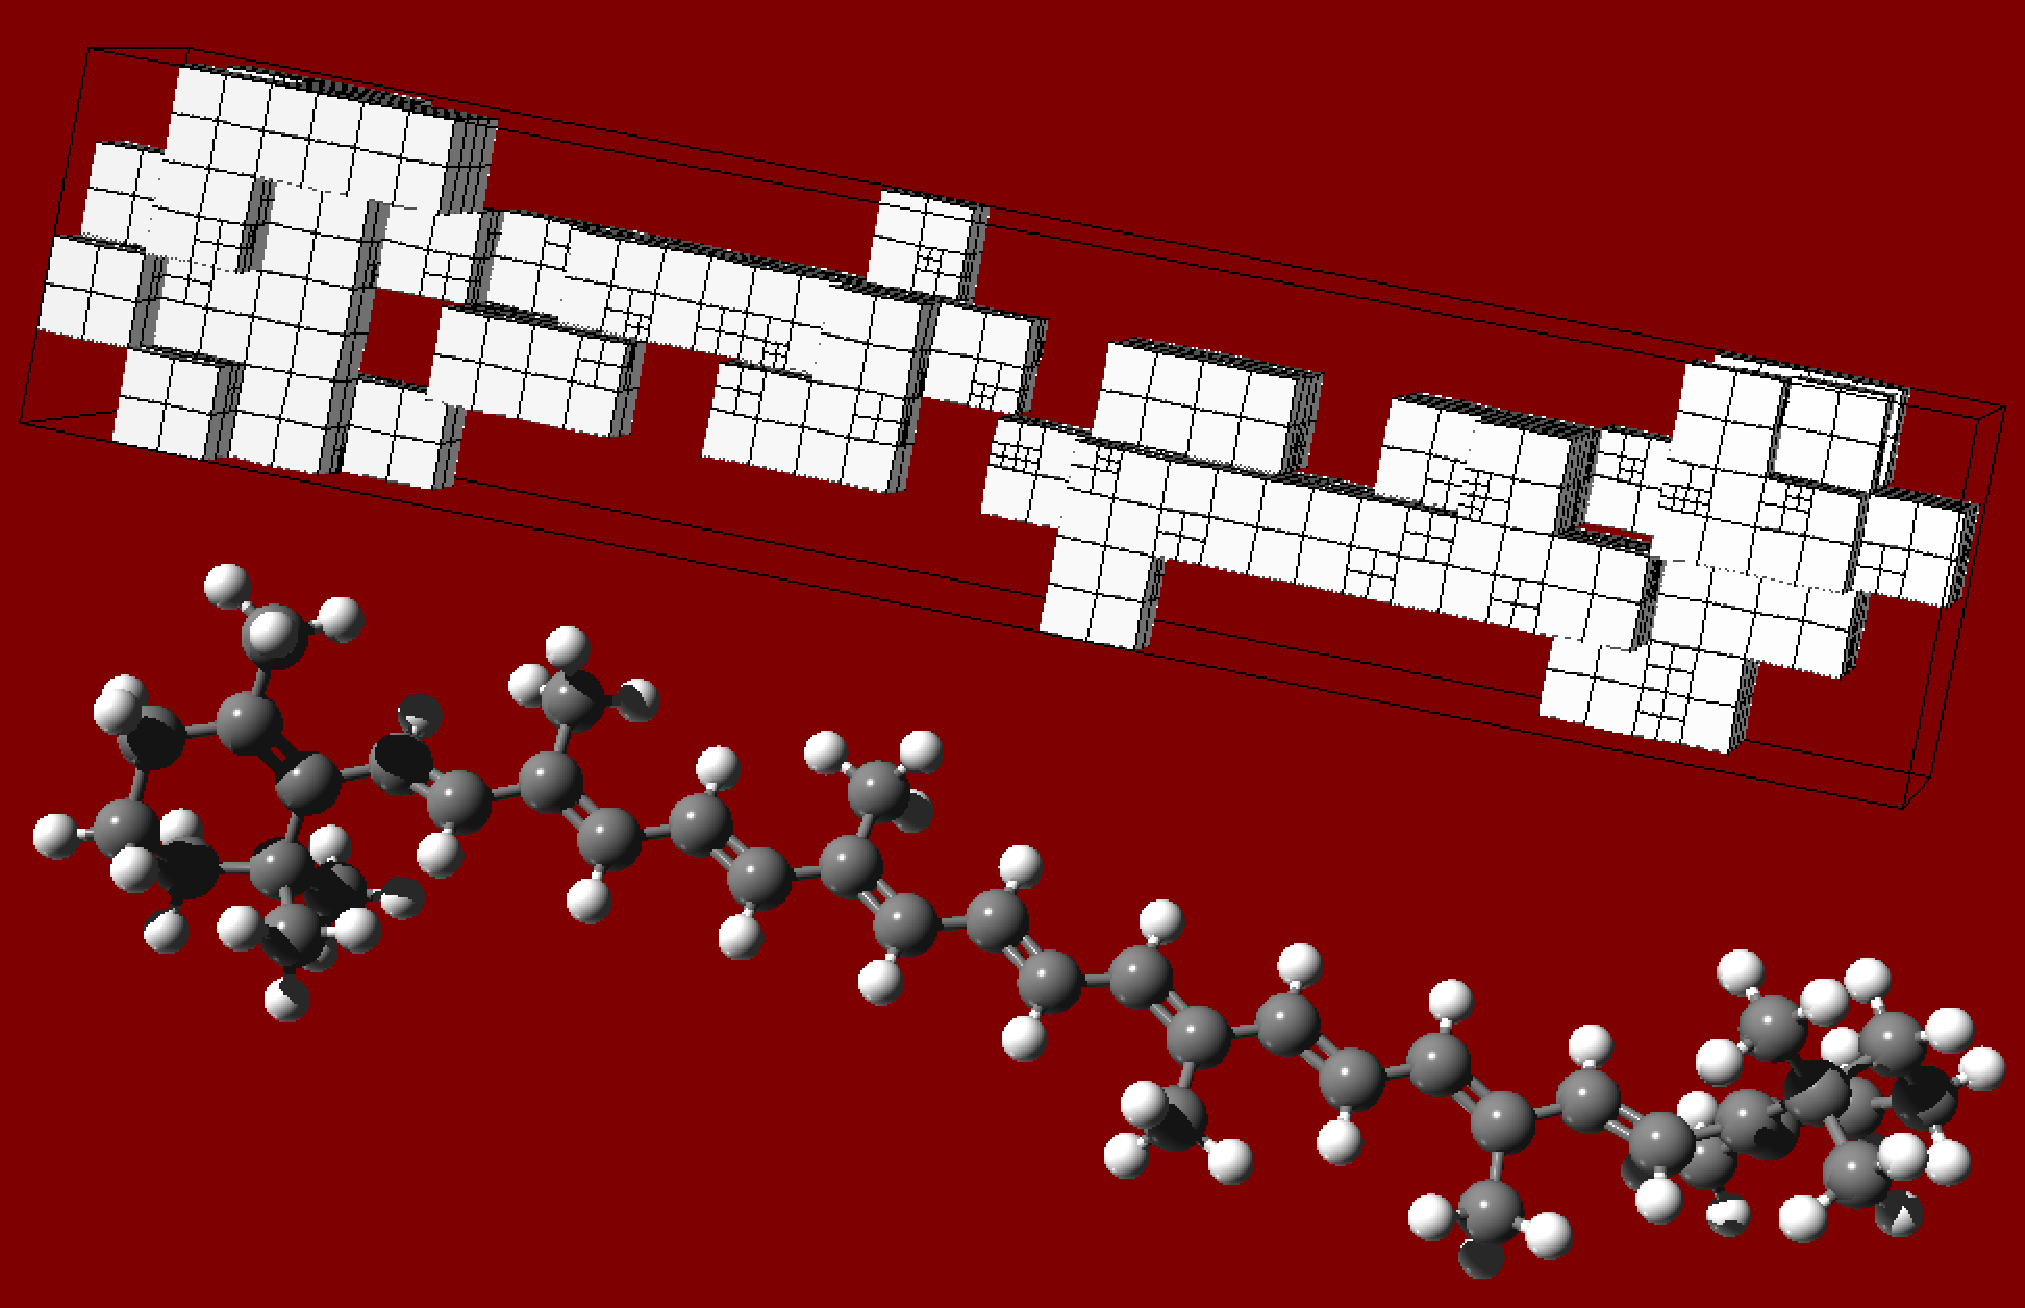
\includegraphics[scale=0.6, viewport = 0 0 1000 650, clip]{figures/adapGrid.pdf}
	\footnotesize
	\\
	\textbf{Figure 2}: Adaptive grid for nuclear potential of carotene
  \end{center}
\end{textblock} 

\begin{textblock}{5}(0,12.3)
  \begin{center}
	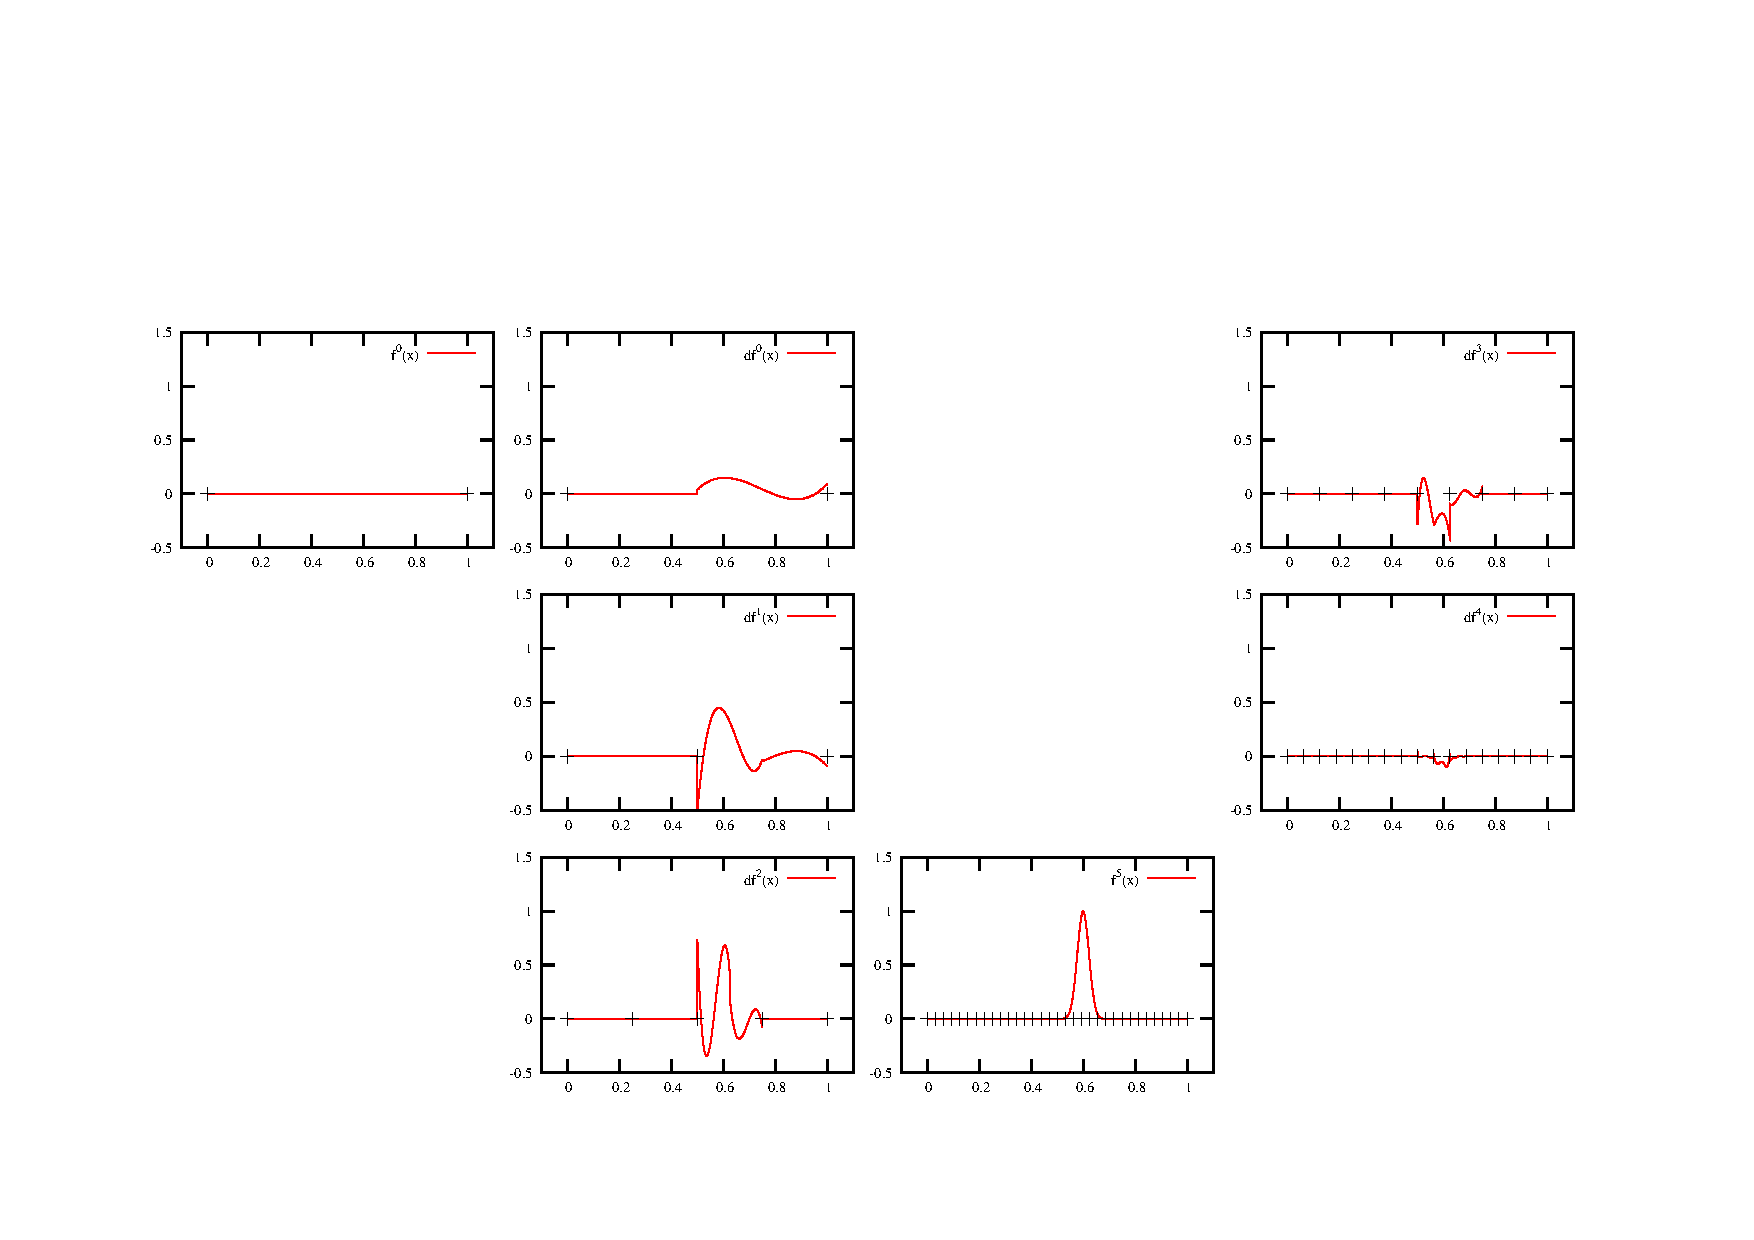
\includegraphics[scale=1.45, viewport = 70 320 410 440, clip]{figures/decomp1.pdf}
  \end{center}
\end{textblock} 

\begin{textblock}{5}(0,13.6)
  \begin{center}
	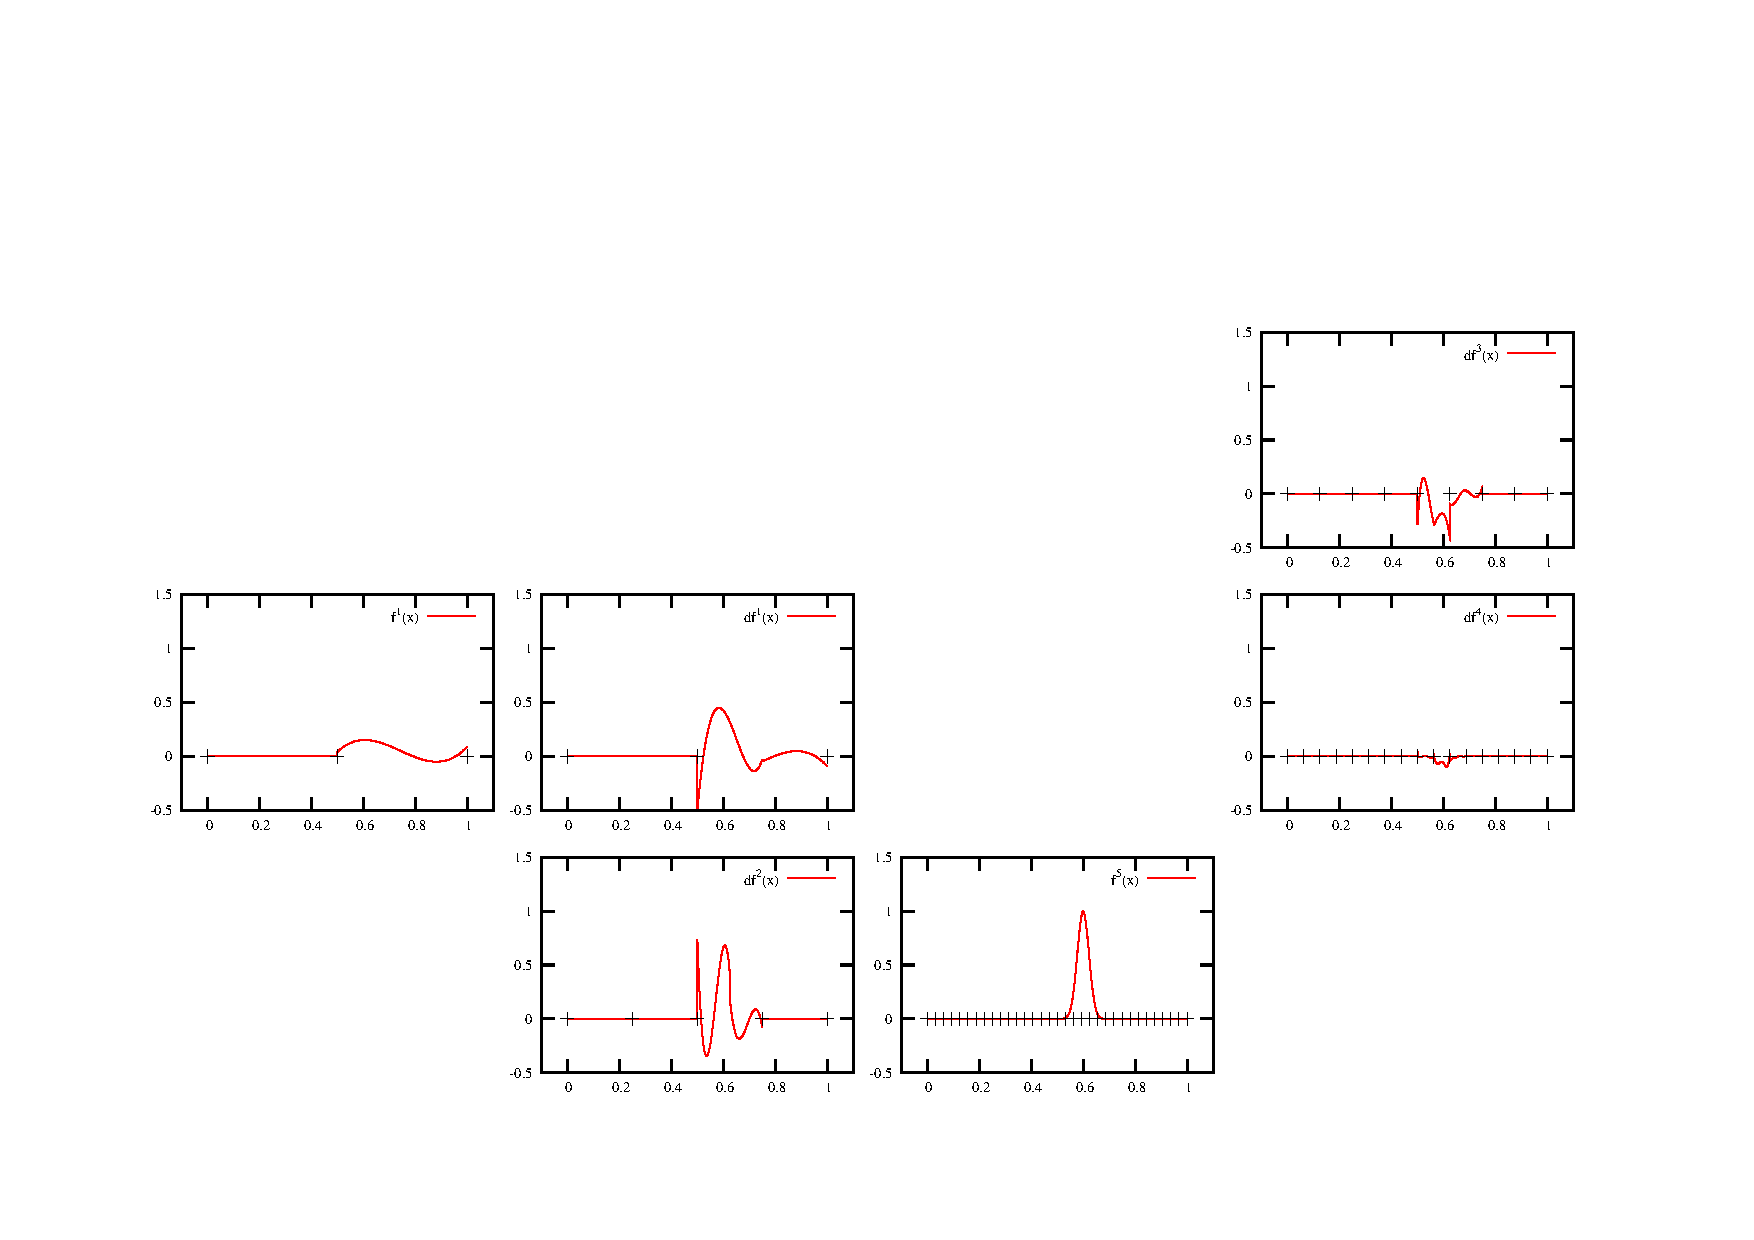
\includegraphics[scale=1.45, viewport = 70 190 410 320, clip]{figures/decomp2.pdf}
  \end{center}
\end{textblock} 

\begin{textblock}{5}(0,15.0)
  \begin{center}
	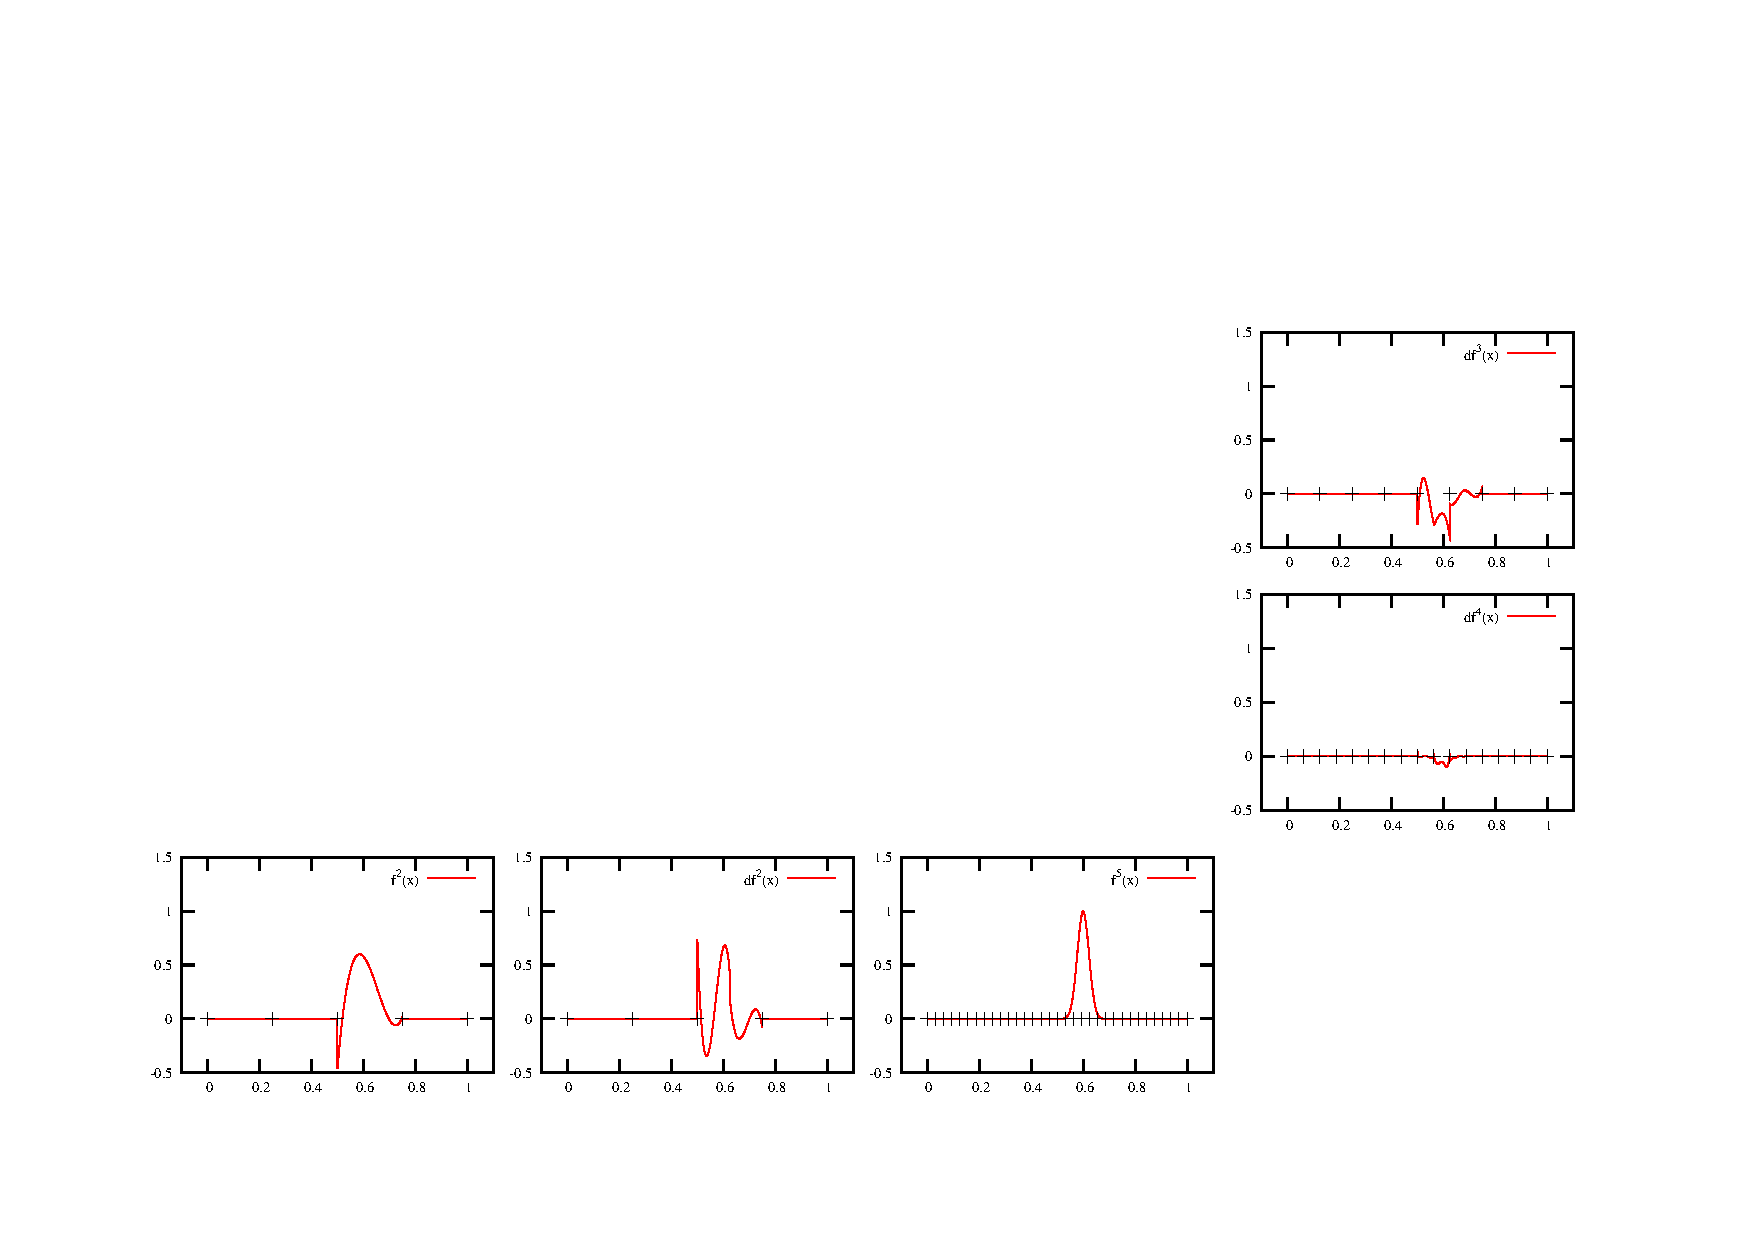
\includegraphics[scale=1.45, viewport = 70 70 410 190, clip]{figures/decomp3.pdf}
  \end{center}
\end{textblock} 

\begin{textblock}{5}(0,16.4)
  \begin{center}
	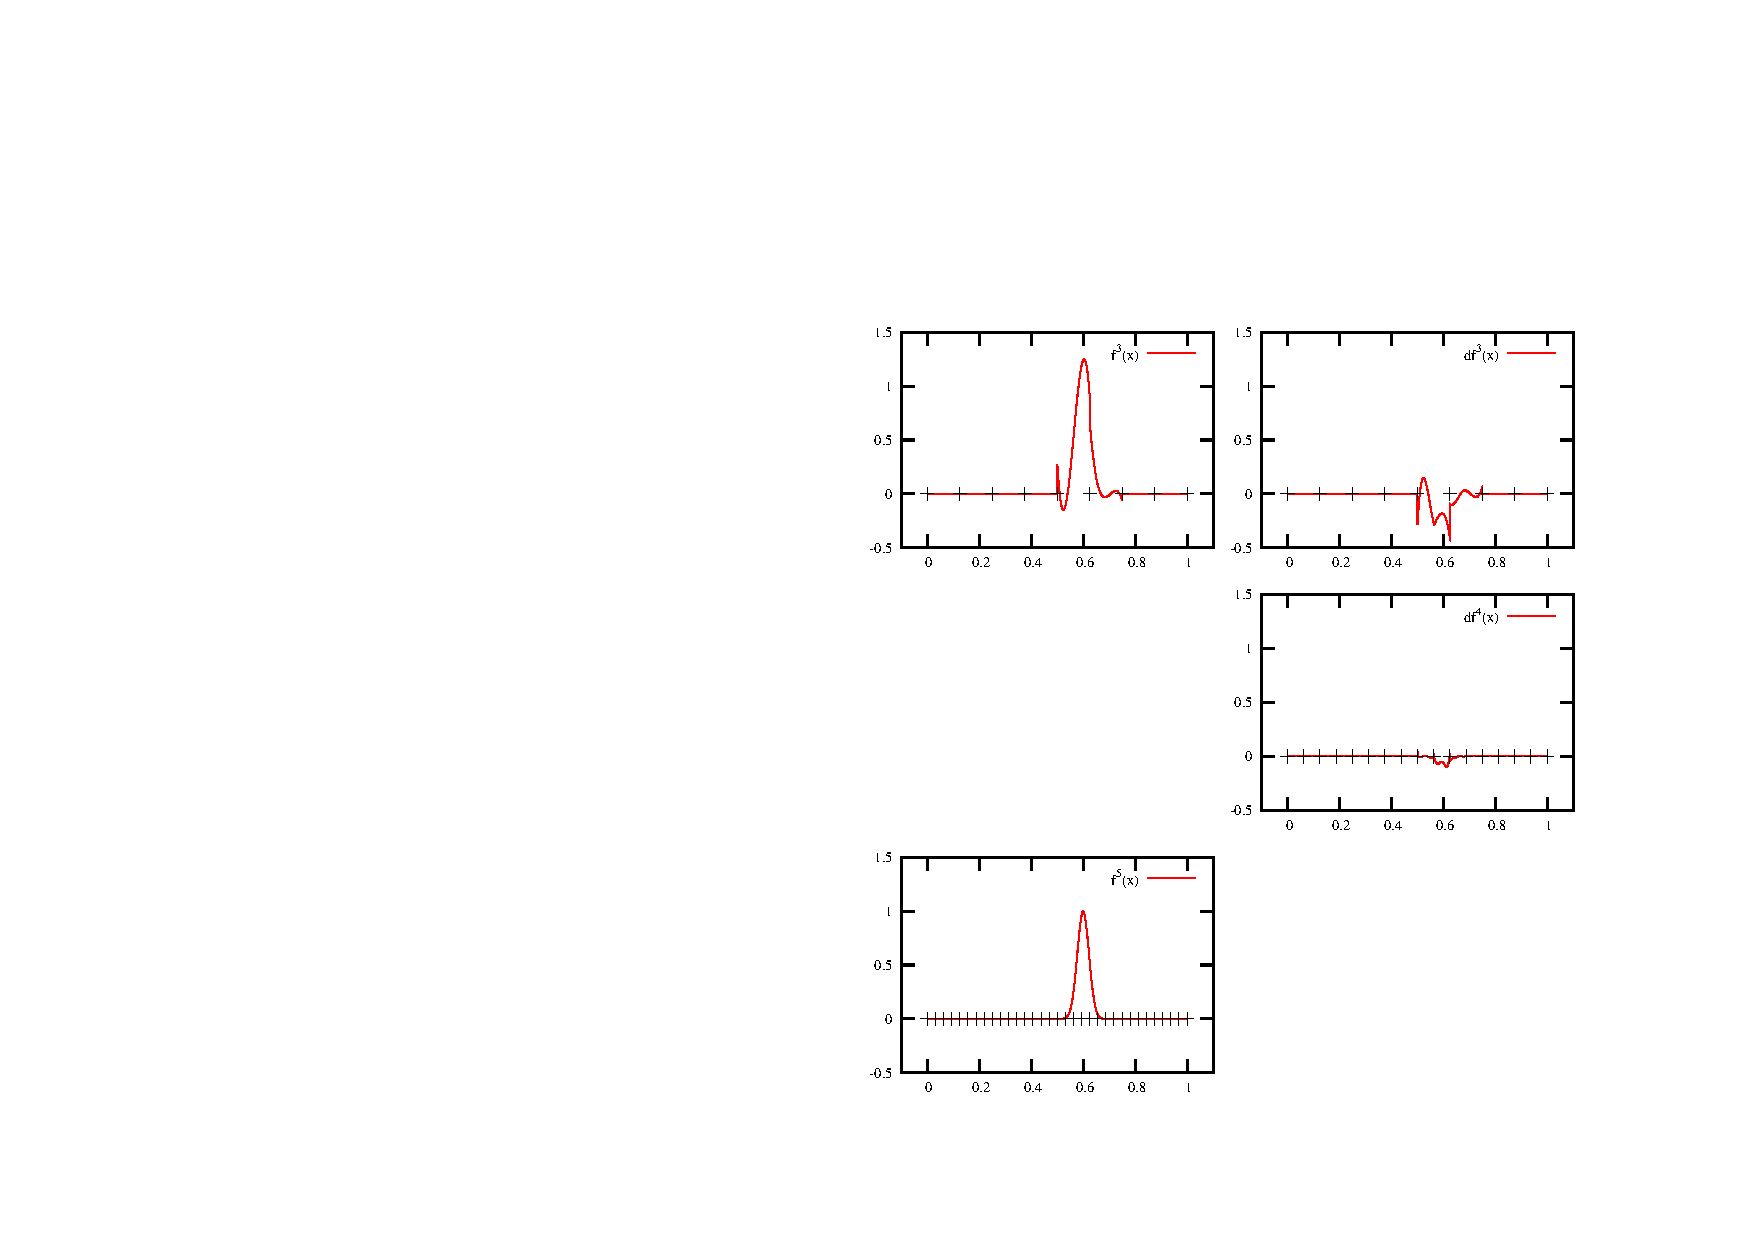
\includegraphics[scale=1.45, viewport = 415 320 755 440, clip]{figures/decomp4.pdf}
  \end{center}
\end{textblock} 

\begin{textblock}{5}(0,17.7)
  \begin{center}
    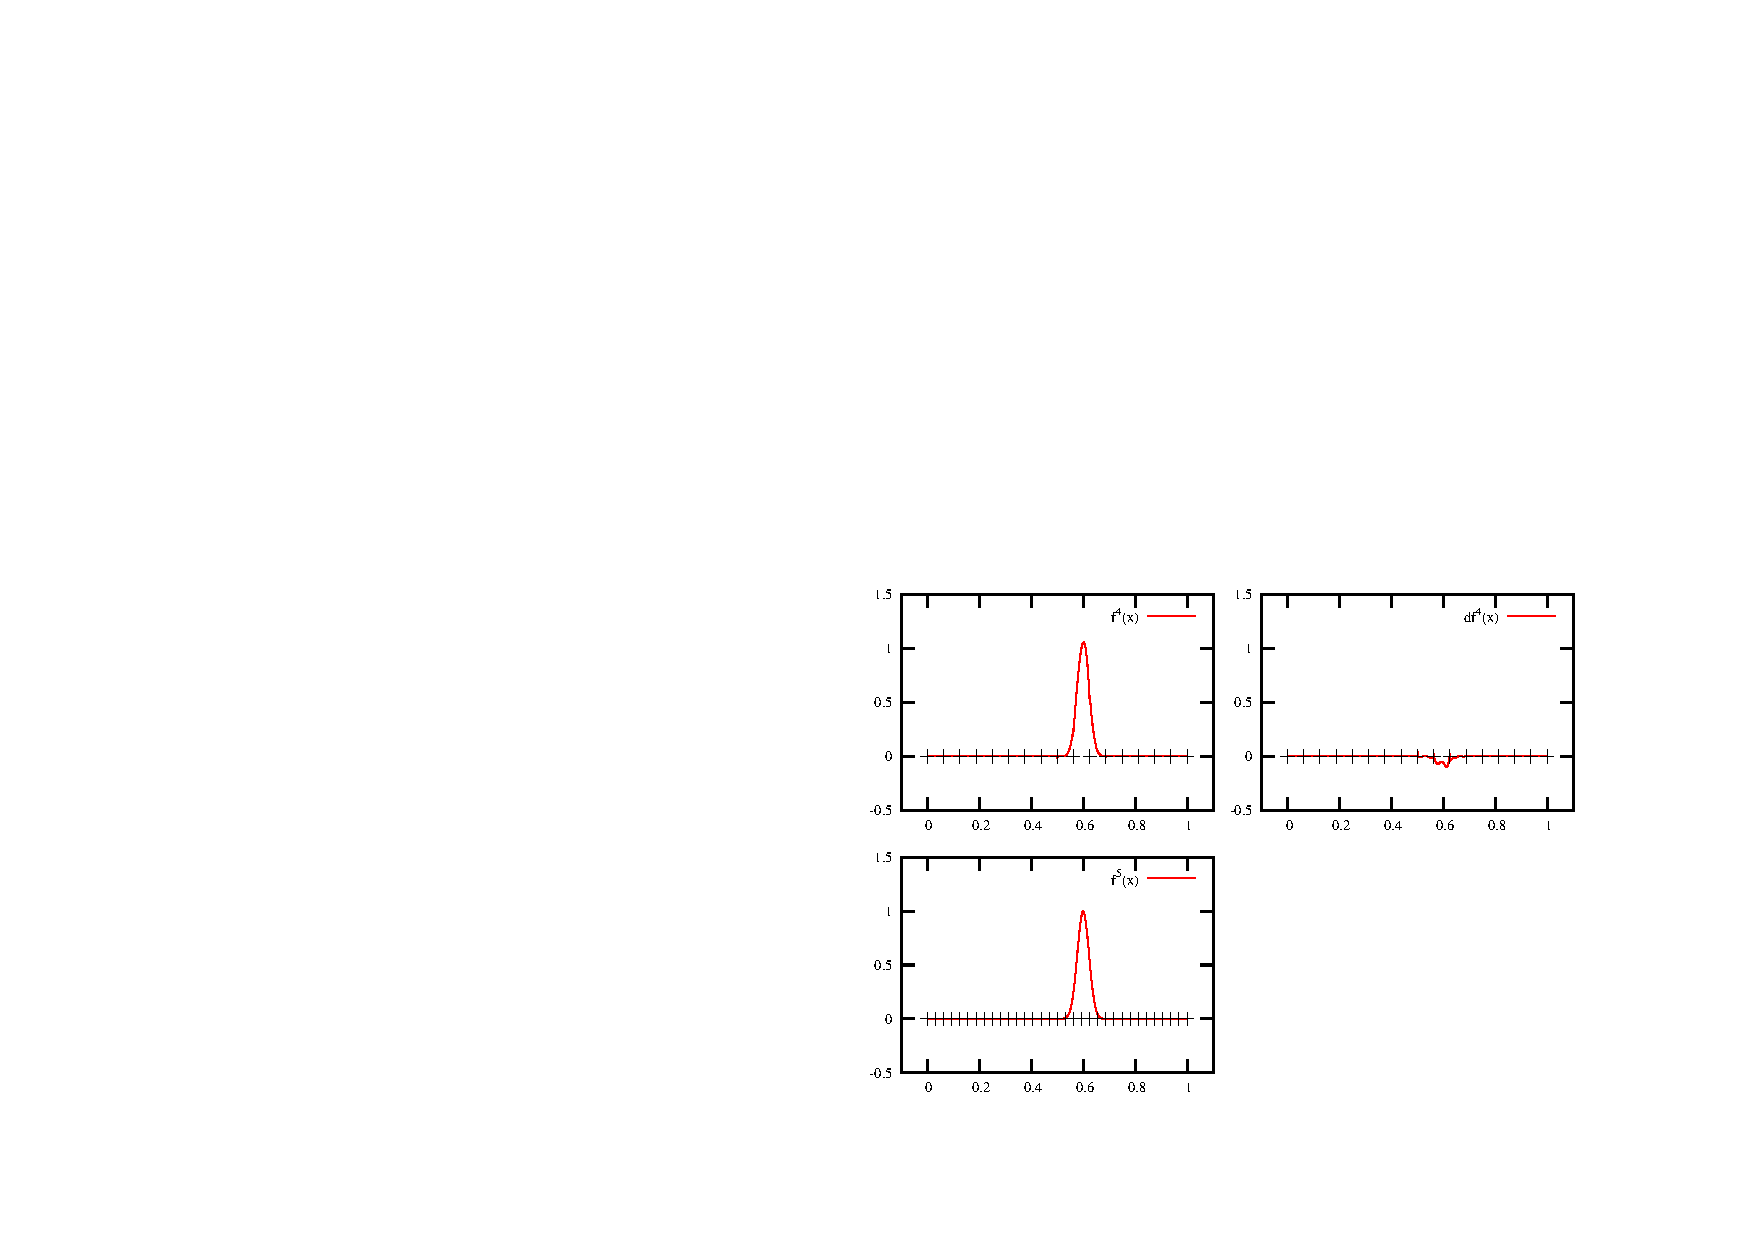
\includegraphics[scale=1.45, viewport = 415 190 755 320, clip]{figures/decomp5.pdf}
    \footnotesize
    \\
    \textbf{Figure 1}: Scaling (left) and wavelet (right) projections of a Gaussian
    function.
  \end{center}
\end{textblock} 

\begin{textblock}{5}(12.2,6.3)
    \Subhead{LDA}
\end{textblock} 
\begin{textblock}{5}(12,6.0)
\footnotesize
\textbf{Table 1}:

\begin{table}
    \normalsize
    \centering
    \begin{tabular}{|l|r@{.}lr@{.}l|r@{.}lr@{.}l|}
	\hline&
	\multicolumn{4}{c|}{Molecule}&\multicolumn{4}{c|}{Molecule}\\
    &	\multicolumn{2}{c}{Energy}&\multicolumn{2}{c|}{Energy}&
	\multicolumn{2}{c}{Energy}&\multicolumn{2}{c|}{Energy}\\
	\hline
	MRChem $10^{-3}$&  0&0& 0&0& 0&0& 0&0\\
	MRChem $10^{-5}$&  0&0& 0&0& 0&0& 0&0\\
	MRChem $10^{-7}$&  0&0& 0&0& 0&0& 0&0\\
    &   \multicolumn{4}{c|}{}&\multicolumn{4}{c|}{}\\
	aug-cc-pV6Z&       0&0& 0&0& 0&0& 0&0\\
	aug-cc-pV5Z&	   0&0& 0&0& 0&0& 0&0\\
	aug-cc-pVQZ&	   0&0& 0&0& 0&0& 0&0\\
	aug-cc-pVTZ&       0&0& 0&0& 0&0& 0&0\\
	\hline
	\end{tabular}
    \end{table}
\end{textblock}

\end{document}
